\chapter{Concept} \label{chap:concept}

\section{General aspects} \label{sec:general-aspects}
In chapter \ref{sec:interaction-i4.0-comp} it became obvious, that \ac{BPM} in \ac{RAMI4.0} is distributed over the different layers. The business layer maps business models in processes, which are linked to certain conditions and prerequisites. This mapping enables the connection of loosely coupled services from the functional layer. Consequently, a control flow is created, that defines the rules for the sequence of the individual activities to be executed. The activities in \ac{BPM} correspond to the functionalities of an \ac{I4.0} component, which are defined in the functional layer and exposed via the submodels of the \ac{AAS}. Essential to the data and business objects used within a process for decision making is the information model. This is specified in \ac{RAMI4.0} by the \ac{AAS} and its submodels. The data and business objects are stored in an interoperable format in the information layer. Storing data in an interoperable format makes it possible to exchange process participants seamlessly without adapting the process itself. However, to be an active process participant, the \ac{AAS} must at least have a representation in the functional layer and be active in terms of their role in value networks. As a result, the information on active participants of a business process can be found in both the functional and business layer. Based on the findings and the defined requirements, a technology-independent architecture can be derived on how \ac{BPM} can be integrated into the \ac{AAS} based on the six layers of \ac{RAMI4.0}. This is illustrated in figure xx. 

In the business layer, the processes representing the business models are described using \ac{BPMN}. Describing processes using \ac{BPMN} has two advantages: On the one hand, this representation creates transparency with regards to the services or activities to be executed, even for non-technical people. Likewise, non-technical people can create and manage the process mappings. On the other hand, using \ac{BPMN}, processes can directly be executed with the help of workflow engines. The integration of the processes modeled into the \ac{AAS} is done via submodels and the properties they contain. Depending on the use case as well as the composition of the \ac{AAS}, the anchoring can take place in different submodels. In the use case of predictive maintenance, the \textit{maintenance} submodel defined by \citeauthor{Cavalieri2020AShell} could be extended by the maintenance process that is necessary in the event of a technical intervention. For this purpose, the activities to be executed would be defined within the process by referencing the corresponding submodels in the \ac{AAS}, such as \textit{set maintenance task} or \textit{get task information}. When implementing workflow engines, however, care must be taken not to create a too strong coupling between the functional layer services and the workflow engine. To this end, it would be worth considering whether the workflow engine should be replace by a message-oriented infrastructure using a message broker.

\section{Design}

The described architecture represents a rather abstract construct, which does not directly indicate the necessary steps for implementation. In the following section, step-by-step instructions will be given on how to implement this. The architecture will be explained on the basis of the use case of predictive maintenance from \citeauthor{Cavalieri2020AShell}. While the paper from \citeauthor{Cavalieri2020AShell} only deals with the modeling of the \ac{AAS} and its submodels, this approach extends their findings by describing a \ac{RAMI4.0} compliant architecture for the implementation of predictive maintenance which conforms to the one elaborated in \ref{sec:general-aspects}. The first step in the implementation is the definition of the composition. This means defining how the assets will be digitized using the \ac{AAS}. In a second step, it must be defined how the connection between the physical and virtual environment can be established with the help of information technologies. Afterwards, for each asset in the system, an information model must be derived that describes the properties and functionalities of the asset, which are then transferred into submodels. In a final step, the processes specified by the business model must be modeled using \ac{BPM}, and the individual activities must be linked to the respective \ac{AAS} or submodel.

\textbf{Step 1: Composition definition}

When defining the composition, the use case to be realized and the assets to be digitized must first be considered. This means that in case of an asset group, the individual components must be identified and considerations must be given to whether they require their own \ac{AAS}. In order to come to a conclusion, it must be evaluated whether the component should be active or passive in terms of their role in value networks and to what extent the functionalities of the asset should be mapped independently of the overall system. As already outlined in \ref{sec:assetadministrationshell}, an asset in \ac{RAMI4.0} can be described by several \ac{AAS}. Likewise, an \ac{AAS} can contain further \ac{AAS}. This results in a multitude of combinations for digitizing assets. For example, in the present case, the milling machine can be implemented as one large \ac{AAS} in which all sub-components, such as the robot's gripper arm are included. It is also conceivable that an \ac{AAS} is created for each individual sub-component, which is then referenced in the \ac{AAS} of the overall system. The difficulty in digitizing assets in \ac{RAMI4.0} using the \ac{AAS} is hence to find the right abstraction based on the scenario the asset is used. 

In the following, three possible forms of composing the milling station will be presented, based on which the advantages of each form will be discussed. Finally, a recommendation for the implementation of predictive maintenance will be given. Figure \ref{fig:aas-modeling-alternatives} graphically shows the three forms.

\begin{figure}[h]
\centering
\subfigure[]{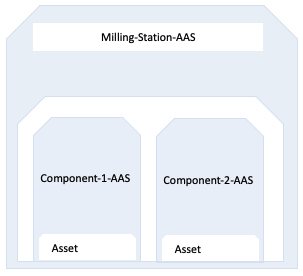
\includegraphics[width=.3\textwidth]{content/pictures/aas_version_1.png}}
\subfigure[]{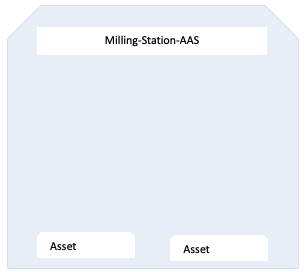
\includegraphics[width=.3\textwidth]{content/pictures/aas_version_2.png}}
\subfigure[]{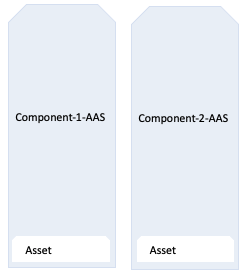
\includegraphics[width=.3\textwidth]{content/pictures/aas_version_3.png}}
\caption{Modelling alternatives for digitizing assets: (a) each \ac{AAS} from the individual components is included in the system \ac{AAS}, (b) all components are covered by a single \ac{AAS}, (c) each component exposes its own \ac{AAS}}
\source{Own illustration}
\label{fig:aas-modeling-alternatives}
\end{figure}

Figure \ref{fig:aas-modeling-alternatives} (a) shows that each component in the milling station is modeled with its own \ac{AAS}. The individual components are aggregated into one \ac{AAS} which is exposed to the network. This type of composition has advantages in reducing complexity while modelling the individual submodels of the \ac{AAS}. This is especially the case if the components of the milling station are delivered by different manufacturers. To this end, each component manufacturer would equip its component with an individual \ac{AAS}. The operator of the asset would then aggregate the individual \ac{AAS} into the milling station \ac{AAS}, which exposes the required properties and functionalities through one interface. In addition to the reduced complexity in modelling, this type of composition has advantages in \ac{SOA}. By addressing one component in the network, communication overhead and complexity can be reduced instead of addressing each \ac{AAS} individually. This type of composition is often found in use cases of plug and produce.

In Figure \ref{fig:aas-modeling-alternatives} (b) all properties and functions of the asset are modeled in one \ac{AAS}. For assets with many sub-components, this type of composition can quickly lead to high complexity in the submodels. However, this type of composition has the advantage, that hardware requirements can be reduced. This is especially the case for \ac{AAS}, that are active but do not have \ac{I4.0} communication capabilities. All functionalities and properties could be provided via one \ac{SBC} or \ac{OPCUA} server.

Figure \ref{fig:aas-modeling-alternatives} (c) shows the type of composition, which has the least coupling between the individual components. It is similar to the composition in \ref{fig:aas-modeling-alternatives} (a), without the aggregation in the milling station \ac{AAS}. For this purpose, each component of the milling station provides its functionalities and properties in the network itself. This type of composition has particular advantages when optimizations are to be realized with regard to latency or information access. For example, it is conceivable that the \ac{AAS} of component 1 is provided by the component itself using \ac{OPCUA} at the edge. The provisioning of component 2's \ac{AAS} can be realized in the cloud, since latencies in communication play a minor role.

\textbf{Step 2: IT-Platform}

\textbf{Step 3: Design of \ac{AAS}}

\textbf{Step 4: Design of business processes}


\section{Roadmap to Industrial Digital Twin}

The introduction of \ac{RAMI4.0}, the \ac{AAS} and the accompanying transformation towards \ac{SOA} can present companies with a challenge. Companies will not be able to adopt directly the development of active \ac{AAS} and adapt their business processes accordingly as described in the previous chapter. Rather, a step-by-step transformation will be required to adapt an organization to the \ac{SOA} proposed by \ac{RAMI4.0} as well as the \ac{AAS}. To this end, the first step is to validate the already implemented measures and derive a development plan. A good framework for classifying and evaluating the current adoption of \ac{RAMI4.0} is provided by the maturity index, developed by \cite[p. 15]{Schuh2020IndustrieAcatech}. The maturity index consists of six successive steps through which adoption of \ac{I4.0} can be evaluated. These are \textit{Computerization}, \textit{Connectivity}, \textit{Visibility}, \textit{Transparency}, \textit{Predictive Capacity} and \textit{Adaptivity}. \textit{Computerization} describes the use of separate, unrelated information technologies, such as \ac{CNC}, to increase efficiency and reduce error rates \cite[p. 15]{Schuh2020IndustrieAcatech}. While \textit{Connectivity} introduces isolated information technologies, \textit{Connectivity} is concerned with the connection of individual production resources on the shop floor via \ac{API}s, which attempt to map the business processes. This can be done with the help of \ac{MES} \cite[p. 16]{Schuh2020IndustrieAcatech}. The two successive steps are referred to by the authors as the digitization, which lay the foundation for the implementation of \ac{I4.0}. The first step towards implementing \ac{I4.0} is \textit{Visibility}. In this step, real-time capabilities are implemented for the assets on the shop floor. The real-time capabilities enable human decision making on based on the current status of the asset. \textit{Visibility} also enables the connection of different data systems in the company such as \ac{MES} with \ac{ERP} \cite[p. 17]{Schuh2020IndustrieAcatech}. The available real-time-data is afterwards aggregated, analyzed and related data sets are linked to it. Therefore, this step is called \textit{Transparency}. The aim of this step is to use Big Data technologies to identify errors, monitor assets and establish impact correlations between the individual data sets.